\documentclass[12pt]{article}
\usepackage[margin=1in]{geometry}
\usepackage{setspace}
\usepackage{graphicx}
\usepackage{amsmath}
\usepackage{natbib} %for citet and citep
\usepackage{syntonly}
\usepackage{esdiff} %for writing partial derivatives
\usepackage{url} %for inserting urls
\usepackage{placeins} % for limitting floats
\usepackage{comment} %for excluding figures
\usepackage{booktabs}
% \excludecomment{figure} % for printing without figures
% \syntaxonly % for quickly checking document
%set document settings

\doublespacing % from package setspacs

\title{The Effect of Oil Price on Field Production: Evidence from the Norwegian Continental Shelf}
\author{Johannes Mauritzen\\
		Department of Economics\\
        BI Norwegian Business School\\
        Trondheim Campus\\
		Trondheim, Norway\\
        johannes.mauritzen@bi.no\\
        \url{jmaurit.github.io}\\
		}
\date{\today}

\begin{document}
 \begin{spacing}{1} %sets spacing to single for title page
	\maketitle

\begin{abstract}
I use detailed field-level data on Norwegian offshore oil production and a semi-parametric additive model to control for the production profile of fields to estimate the effect of oil prices on production.  I find no significant evidence of a concurrent reaction of field production to oil prices, though a modest lagged effect is found of the magnitude of approximately 2 to 7\% for a 10 dollar per barrel increase in the real price of oil.\\
Keywords: Oil production,Oil Prices, Norway, Generalized Additive Model.
Words: 7000
\end{abstract}

\thanks{}
% JEL Codes: Q4, L71
 \end{spacing}

\section{Introduction}

For most of the last century, crude oil has been the world's single most important and valuable fuel source.\footnote{Oil is the world's largest single energy source, consisting of approximately 33\% of total energy consumption in 2013 as well as the most valuable in terms of market price per unit of energy \citep{british_petroleum_statistical_2013}} Naturally, questions of how the oil price affects the world economy as well as how oil production reacts to the oil price have been fundamental topics in Economics. Recent volatility in the price of oil has made this an especially relevant topic. 

Oil and gas supply, especially in difficult and expensive offshore areas, is the product of an often lengthy and complex chain of conditional investment decisions. Starting with the exploration phase, where a potential oil-producing region or "play" is explored, leases are acquired, prospects are identified and exploration wells are drilled. In the case of a significant hydrocarbon find, a field is appraised to judge size, difficulty and in turn profitability. For fields seen as sufficiently profitable, a development stage commences, where a detailed drilling and production plan is drawn up and submitted to obtain permits and regulatory approval. Operating agreements are signed and subcontractors acquired for offshore construction and well development. Finally, at the end of this multi-year process, a build-out can commence, where full production capacity is built out as fast as possible, followed by an extended depletion phase. All of this consists of what is referred to as upstream activity, with steps such as shipping, refining and trading, among others, making up an equally complex down-stream process. \footnote{\citet{lefler_deepwater_2011} provides an accessible guide to the offshore petroleum exploration and production industry.} 

A large body of economic litterature exists on the complex chain of investment and production decisions made in the upstream oil and gas industry. This article looks at the limited, but important topic of the effect of price on production from active offshore fields, where a significant gap exists in the literature.  

While numerous studies have taken up the issue of how the price of oil affects searching for new fields as well as total oil production at both the regional and global level, few studies exist of the effects of oil prices on oil production at the field level.  The studies that do use field- and well-level data, such as \citet{rao_taxation_2010}, often use data from on-shore installations.  However an increasing amount of the world's oil production comes from hard-to-reach offshore fields.  Production from challenging offshore environments is substantially different in character than from on-shore installations.

The effect of oil prices on producing fields is an important topic in understanding the mechanisms of how total oil supply reacts in response to price. The response of oil production in existing fields is especially important now as many of the major oil-producing areas, like the Norwegian Continental Shelf are mature and an increasing share of total investment will be directed at capacity enhancement in producing fields rather than new field developments. Figure \ref{investment} shows that investments in producing fields makes up a large and growing share of total investment, nearly dwarfing investments in searching, exploration and new build-outs. How production from mature fields will respond to changes in oil prices has major implications for the oil industry, the state finances of oil-producing countries and long-run oil price formation.

\begin{figure}
	\center
	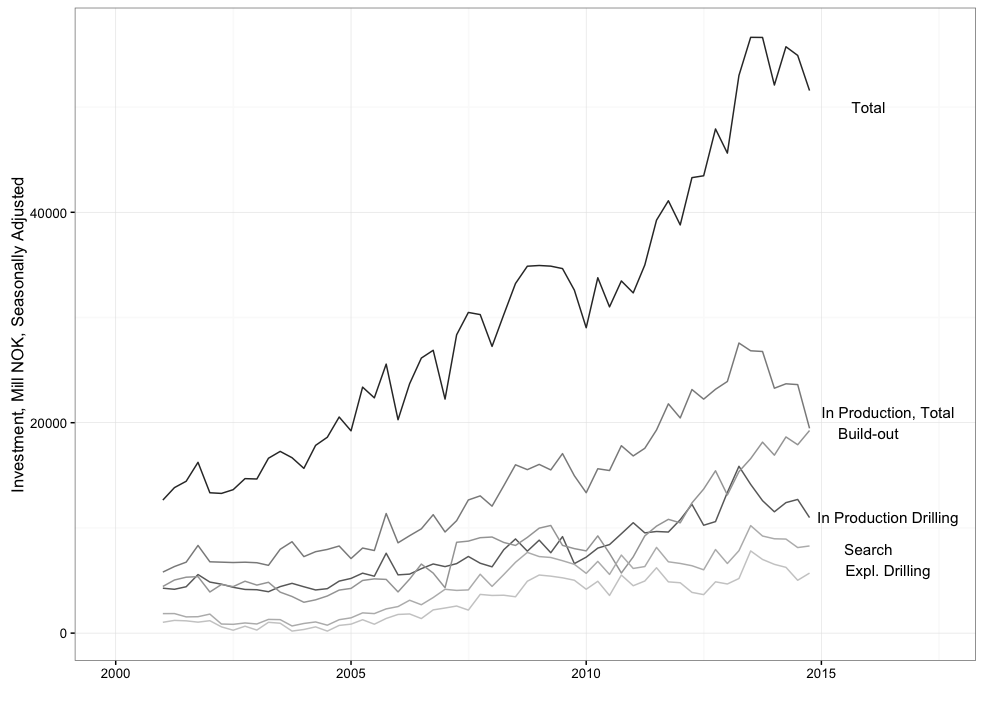
\includegraphics[width=.9\textwidth]{figures/investment.png}
	\caption{The figure shows investment (millions NOK) in the oil and gas extraction industry on the Norwegian Continental Shelf. A large and growing share of total investment goes into fields that are already producing as opposed to investment in search, exploration and build-out of new fields.}
	\label{investment}
\end{figure} 

The question of the effect of oil prices on production and the more general question of optimal oil extraction has spawned a large theoretical literature dating back to the seminal work of \citet{hotelling_economics_1931}. \citet{krautkraemer_nonrenewable_1998} provides a good overview. At a basic level a central idea of much of this theoretical work is that with a non-renewable resource, production is a decision that involves a significant opportunity cost: more production in the current period means less production in future periods.  Within these frameworks, prices and expectations of prices become important variables in the production decision. A simple Hotelling model suggests that a producer would immediately change their production in response to a change in oil price in order to dynamically optimize the total extraction.

But in practice, the question is not as clear cut.  Production on the Norwegian Continental Shelf - as well as most other offshore production areas - has extremely high fixed and operating costs.  Keeping spare capacity available in order to adjust to changing oil prices might simply be too expensive.  Instead, producers may find it more beneficial to use storage and financial instruments in order to hedge short-term price movements. Higher oil prices may still lead a producer to invest in increased capacity.  Since lag times are significant in the offshore sector, we would then expect to see a multi-year lagged effect of prices on production.  

However even with the question of lagged production and investment, some ambiguity exists.  \citet{mohn_efforts_2008} suggests and finds evidence for the idea that in periods of high oil prices offshore producers will invest more in risky wild-cat drilling in search of new fields. But when prices are low, they tend to concentrate investments in lower-risk ventures, like expanding production in existing fields. If this effect were to dominate, then it may even be plausible that a fall in prices leads to an \emph{increase} in production. Though the converse - an increase in prices leading to reduced production - is unlikely.  

%Implications for theories and explanations for understanding of the price mechanism and %the role of speculation.  Hamilton block quote.  

For such a prominent subject, the lack of research on the role of price in oil field production is striking. Two main factors likely contribute to the limited literature - the availability of data and the non-linear time profile of field production.  Large private oil companies, notably the “super majors” and state-owned oil companies have historically accounted for the vast majority of oil production and reserves. \footnote{See for example the economist article titled Supermajordämmerung from August 3rd, 2013: \url{http://www.economist.com/news/briefing/21582522-day-huge-integrated-international-oil-company-drawing}} These entities tend to consider field-level data as either company or state secrets.   

However, over the last few years, a movement towards making the petroleum and other extractive industries more transparent has taken form.  The Norwegian government has been on the forefront of this movement and increasingly committed itself to transparency in the petroleum sector. \footnote{See \url{http://www.regjeringen.no/en/sub/eiti---extractive-industries-tranparency/about-eiti.html?id=633586}} Over the last several years, detailed data on most aspects of the country's oil industry has become openly available.  

In this article, I use historical production data from nearly all 77 currently or formerly oil-producing fields on the Norwegian Continental Shelf in order to estimate the effect that prices have on oil production. 

By looking only at the effect of price on fields that currently or previously have produced oil, I am limiting the scope of this article.  The effect of oil prices on total production over an extended period of time is due not just to reactions in production in existing fields but also increased searching for new fields.  In fact, an implication of this work is that much of the total production response from higher oil prices is likely from increased searching as well as production from previously un-economic fields.

The main finding in this article is that oil production at the field level has no significant reaction to concurrent changes in the oil price.  A modest effect can be detected at a lag of between 2 and 4 years of between 2 to 7\% increase in yearly production for a 10 dollar increase in the price of oil.

% Price appears to have the most significant affect during the planning and build-out stage.  In the depletion phase of production, price is found to have little to no significant effect.  

The main methodological problem is the non-linear production profile of oil fields.  Once full-scale extraction is started in an oil field, pressure in wells will start declining. Compensating measures such as gas and water injection have been successful, but their impact is temporary. In turn production rates will therefore inevitably decline.

More so, major oil field discoveries, starting times and in turn production are correlated across fields as the top panel of figure \ref{oil_decline} shows with the production profile of the 10 largest Norwegian oil fields.  The result is a total production curve that is bell-shaped over time as in the lower panel of figure \ref{oil_decline}.  Since the oil price series is autocorrelated and non-stationary, failure to properly account for the production profile will lead to spurious estimation of the price terms in a regression.

\begin{figure}
	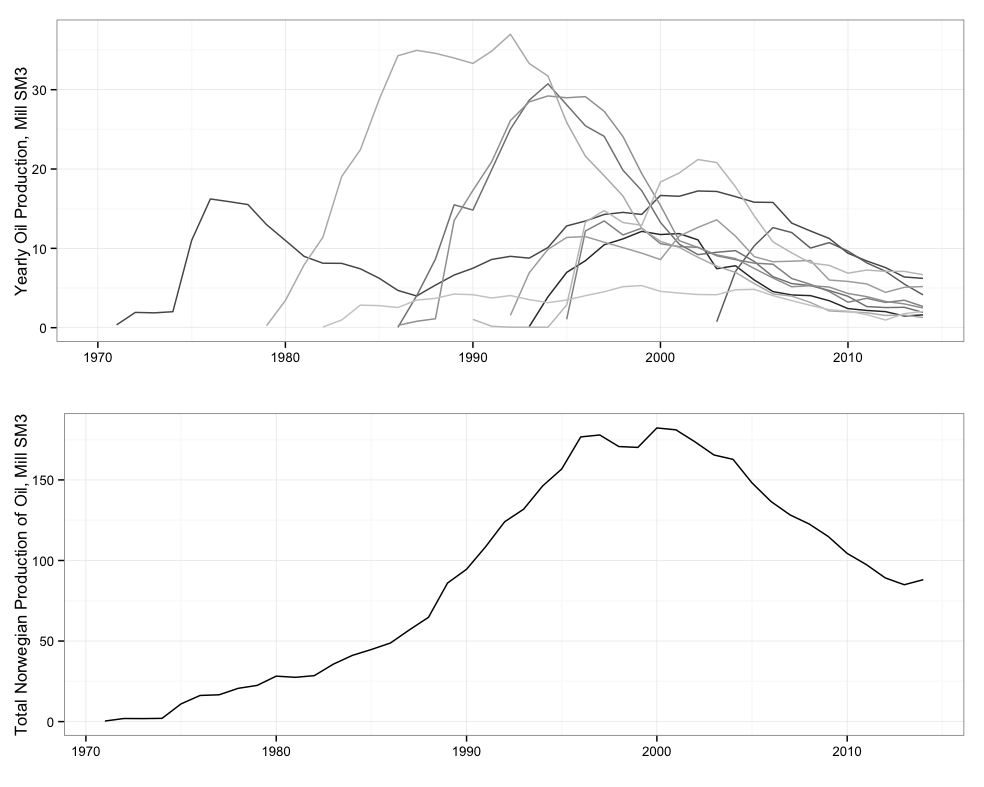
\includegraphics[width=1\textwidth]{figures/oil_decline.png}
	\caption{The top panel shows the production from the largest 10 oil fields on the Norwegian Continental Shelf, whose starting times are temporally correlated with each other.  The total production over time is bell-shaped, as shown by the bottom panel.}
	\label{oil_decline}
\end{figure}

The direction of this bias can be gleaned in figure \ref{oil_decline}.  High oil prices were present at periods of relatively low production in the late 1970s and early 1980s as well as over the last 10 years, however real prices reached some of their lowest levels at the same time as the top of production around the year 2000. These oil price dynamics almost certainly affected investment decisions in the industry and in turn total production \citep{osmundsen_is_2007}, \citep{aune_financial_2010}. However the inverse contemporaneous relationship at the field level is entirely coincidental, but will heavily bias the estimation of the effect of price on production if field production profiles are not properly accounted for. 

As a solution I use a semi-parametric model within the Generalized Additive Model frameworks of \cite{hastie_generalized_1990}.  Here I use both a cubic regression spline and a two-dimensional thin-plate regression spline to account for the general non-parametric shape of the production profile, while allowing price to enter the equation linearly. I also attempt to control for the effects of varying production costs and the effects of technological change.

The results suggest that little to no concurrent effect of oil prices on production exists.  However I estimate modest effects on the first through fourth lagged terms. These results are in line with an understanding of the industry as being highly capital intensive with high operating costs.  Maintaining spare capacity in order to adjust to changing oil prices is likely prohibitively expensive.  Instead, production is increased through investment, which may take up to several years to show an effect.

\section{Econometric Litterature on The Effect of Oil Price on Production}

%For modeling aggregate oil production, shape-fitting models, notably \citet{hubbert_energy_1962} and more recently advocated by \citet{deffeyes_hubberts_2001}, have had some success in estimating the timing of peak production at the regional and national level, but they tend to seriously underestimate the total recoverable resource of oil-producing regions and the models can be shown to be fundamentally misspecified \citep{boyce_prediction_2013}.   Simulation type studies where aggregate oil production is modeled through an often complex combination of physical and economic processes also exist in the geo-engineering literature, but their usefulness tends to be weighed down by their complexity as they require quite detailed data and specific assumptions about functional form that can be difficult to justify \citep{brandt_review_2010}.

An extensive litterature exists that attempts to estimate the effect of oil prices on regional or global oil supply. Early econometric attempts, like \citet{adelman_fea_1975} often made the assumption that the price contained all relevant information, ignoring the role of geophysical limits at the regional level. \citet{hamilton_oil_1983} showed that macroeconomic events could not fully explain movements in oil prices, rejecting the notion that prices contained all relevant information to oil supply. \citet{kaufmann_oil_1991} presents a relatively early attempt at combining both economic and geophysical aspects in an emperical model of oil production in the US. The author used a Hbbert-like \citep{hubbert_energy_1962} shape-fitting model to capture regional geophysical dynamics, using the residuals to model the effects of price on production. The author predicted that depletion and reduced oil supply from the lower 48 states would continue - a prediction that proved mostly accurate up until the technological revolution of fracking and shale oil extraction. 

A similar analysis combining econometric models with shape-fitting models by \citet{cleveland_forecasting_1991} also led to pessimistic forecasts of future US production. Further refinements of these were done by, among others, \citet{pesaran_forecasting_1995}  and \citet{moroney_integrated_1999}. \citet{kaufmann_oil_2001} present an extension and generalisation using a Vector Error Correction Model (VECM) that relaxes the assumption that firms produce their fields in order of decreasing quality and also includes institutional factors in US oil production. They claim that they are able to account for most of the price variation between 1938 and 1991.

\citet{adelman_mineral_1990} and \citet{adelman_modelling_1993} takes an opposing view, using cointegration and causality testing to argue that scarcity, and in turn geophysical forces had little to do with the oil price movements of the 1970s and 1980s. Instead Adelman argues that cartel behavior of low cost producers likely stood behind increasing oil prices. \citet{lynch_forecasting_2002} provides a fuller overview of these competing strands of litterature. 

The economics litterature on petroleum production tends to be overweighted towards studies of the US, but some global studies have also been attempted. \citet{watkins_world_1998} attempt to estimate supply functions for 41 countries by estimating the relationship between the price of undeveloped reserves and reserve additions over time. Based on the aggregated estimates, they argued that fears of increasing global scarcity at the time were overblown. 

\citet{farzin_impact_2001} attempts to estimate the price elasticity of added global reserves and finds a small positive elasticity.  \citet{ramcharran_oil_2002} estimates a total supply function of oil from several OPEC countries based on data from 1973 to 1997.  The author finds a negative price elasticity for several of the countries, and interprets this as evidence of producers targeting revenue.  However since the author does not take into account the production profile of oil fields and the spurious correlation that can arise with autocorrelated prices, these estimates come under considerable doubt. \citet{ringlund_does_2008} estimates how rig activity reacts to changes in oil prices in non-Opec countries, and finds substantial heterogeneity based on the structure of a country's oil industry. Though in the long run, they find an average elasticity of close to one. 

On the surface, this article fits well into the previous econometrics litterature on petroleum supply in that there is a focus on establishing and decomposing the effects of geophysical and economic forces. However, most of the above articles focus on total long-term regional oil supply, which as I mention above, is the result of an extensive chain of decisions from surveying of a potential play, exploration drilling, to production. This article, on the other hand, is considerably narrower in scope - focusing exclusively on production in active fields. While ambiguity exists on whether geophysical forces and scarcity are significant factors that need to be controlled for in the long term regional perspective, they are without question dominant factors at the field level.

Microeconomic aspects of oil supply have more recently come to the fore. \citet{kellogg_effect_2014} studies the effect of oil-price uncertainty on drilling and exploration. The author finds that oil exploration firms in Texas approximately respond as real-option theory would predict when it comes to the timing of drilling.  A model and test using data from North Sea producers on the UK continental shelf by \citet{hurn_geology_1994}, on the other hand, fails to find evidence that the variance in the oil price affects the timing of oil field development.  

I do not attempt to directly model uncertainty, however given that the investments needed to increase oil production in an existing field are to a certain extent irreversible and that oil prices are highly volatile, the results can and probably should be interpreted with the real options framework in mind.  

Studies using detailed Norwegian data on offshore activity also exist, though the focus has mainly been on exploration and drilling.  \citet{mohn_exploration_2008} finds that long-term changes in the oil-price has a strong effect on exploratory drilling though little effect is measured from short-term changes in the oil price. \citet{osmundsen_exploration_2010} analyses drilling productivity over time on the Norwegian Continental Shelf while \citet{mohn_efforts_2008} finds that higher oil prices leads to higher reserves as well as that oil prices affect producer risk-preferences - with higher prices leading to lower success rates but larger discovery size. \citet{mohn_elastic_2010} presents a thorough econometric analysis of the role of economic and policy factors in oil exploration and reserve additions, as well as a useful summary of exploration and production on the Norwegian Continental Shelf.

Most of the microeconometric articles analyzing the petroleum industry, like the ones mentioned above, focus on issues of exploration, drilling, and rig activity. Microeconomic studies of production from operational fields are more sparse. \citet{black_is_1998} tests the relevance of “nesting” a structural empirical model of profit maximization that takes into account oil prices into a typical geo-engineering model of oil field production.  They find strong evidence that taking into account profit maximization - and implicitly price - substantially improves the fit compared to a purely geo-engineering model. The major limitation of their methodology is that they are only able to test whether including economic factors like price affects the fit of the model but are not able to give an estimate of the magnitude of the effect. Methodologically, the paper also relies heavily on strict assumptions about the functional form of both the geo-engineering and economic aspects of their model.  By taking a more flexible, semi-parametric approach to modeling oil field production profiles, this article avoids problems with overly restrictive assumptions. 

\citet{rao_taxation_2010} uses data on onshore oil wells in California to estimate the effects of tax changes and price controls. The author finds that short-term tax changes caused small, but significant re-timing of production from oil wells.  These findings are generally consistent with the findings of this article, though the author finds a concurrent effect of changes in taxation on production while I do not find any concurrent effect of prices on production. The significant differences in cost and complexity between operating offshore and onshore likely account for the different results.  How producers react to a short-term tax change as opposed to a change in price also likely differs.

\section{Oil Production on the Norwegian Continental Shelf}

The first commercial oil well in Norwegian continental waters was discovered in December of 1969 in what became the Ekofisk oil field. Most of the largest fields in the North Sea were found relatively early on while more recent finds have tended to be smaller - a pattern typical of oil producing areas called creaming. A major exception to this trend was the recent find of the Johan Sverdrup field which is estimated to have approximately 300 million Standard Cubic Meters (SM3) of recoverable oil. \footnote{The Johan Sverdrup field is estimated to begin producing oil in 2019 and is not present in the data set used for the analysis.}

Exploration in the Norwegian Sea was opened in the early 1980’s and the first commercial field started production in 1981.  While several mid-sized fields have been discovered, the Norwegian Sea has generally disappointed in terms of commercial oil finds.  

Norwegian waters in the Barents Sea have also been open to exploration since the 1980s, however up until recently only a few, small finds were made and none came into commercial production.  Recently several significant oil and gas finds have been made in the Barents Sea - notably the oil field Goliat and the large gas find Sn\o hvit, which are both currently under development but not yet producing.  The agreement between Norway and Russia in June 2011 settling a long-running dispute over the maritime delimitation has also given a boost to new exploration in the region.  

Profits from oil and gas production in Norway are subject to a resource tax of 51 \% on top of the ordinary income tax of 27 \%, thus income from petroleum production is taxed at a total marginal rate of 78 \%.  The central government also receives revenues through its majority ownership stake in Statoil. In addition, a wholly state-owned company, Petero, manages the development licenses that the state retains - referred to as the State's Direct Financial Interest (SDFI).

The tax system is also designed to be neutral, that is a field that is profitable before tax should also be profitable after tax. This is accomplished by only taxing the net-profits of oil companies, allowing companies to deduct investment costs and deduct and carry forward losses.\footnote{The Norwegian Oil and Gas industry group Norsk Petroleum provides a fuller overview: \url{http://www.norskpetroleum.no/en/framework/petroleum-tax/}}

The over-all tax rate has been fairly constant through the history of Norwegian petroleum production, however several important changes related to the tax code have occurred.  In 1991 a C02 tax was introduced, and in the year 2012 the tax was doubled.  But this was mainly levied on the use and import of petroleum products.  In the offshore sector it was levied on the burning of oil and gas and thus the main effect was on the practice of flaring natural gas that could not be transported and sold commercially.

More important to the offshore sector were accounting changes that were implemented in 2002 and 2005, which were meant to encourage new entrants by allowing losses to be carried forward for tax purposes and by introducing a rebate on the tax-value of losses associated with searching and drilling.  In general though, these rules mainly affected searching and discoveries of new fields rather than production from existing fields and I do not control for the tax changes in my model.  More information on taxation and revenues from the offshore sector can be found at the website of the Norwegian Ministry of Finance. \footnote{\url{http://www.regjeringen.no/en/dep/fin/Selected-topics/taxes-and-duties/bedriftsbeskatning/Taxation-of-petroleum-activities.html?id=417318}}

Rights to explore and eventually produce on the Norwegian Continental Shelf are based on a system where the government announces geographic blocks that will be opened to oil exploration and production subject to production licenses.  Production licenses are initially granted for between 4-6 years subject to requirements that firms are actively searching in their awarded blocks.  If oil or gas deposits are proven then the production license can be extended for up to 30 years.  In general, the frameworks are fair, predictable and stable for companies who find commercially extractable oil deposits and regulatory interference is unlikely to be the cause of any observed changes in production from existing oil fields.  For more information see the website of the Norwegian Petroleum Directorate. \footnote{\url{http://www.npd.no/en/Topics/Production-licences/Theme-articles/Production-licence--licence-to-explore-discover-and-produce-/}}

\section{Data}
Norwegian oil field production data is obtained from the website of the Norwegian Petroleum Directorate.\footnote{http://factpages.npd.no/} The data I use includes nearly all current or formerly oil-producing fields, from 1971 through 2014. Production data is available at a monthly frequency, though I choose to aggregate up to yearly values both to smooth over seasonality as well as short-term volatility of output due to factors such as weather or technical issues that are not relevant for this article. 

In addition to data on field-level production, I also have access to data on estimates of total recoverable reserves as well as estimates of total in-place oil for each field. The use of total recoverable reserves is complicated since it is dependent on the price of oil and thus endogenous in the analysis. Therefore, as a proxy for the size of the fields, I use estimates of geological in-place oil which is not a function of economic factors. The left panels of figure \ref{data_descriptives} show the histograms of field sizes as measured by estimates of recoverable oil and in-place oil. 

\begin{figure}
	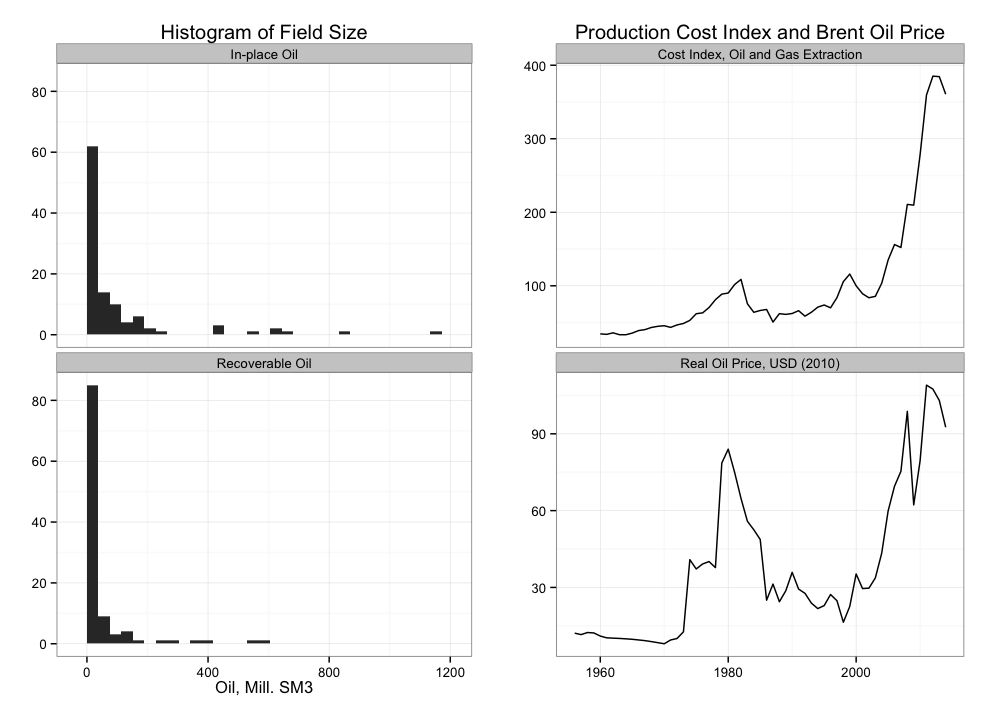
\includegraphics[width=1\textwidth]{figures/data_descriptives.png}
	\caption{Data descriptives. The left panels show histograms of estimates of recoverable oil and in-place oil by field. The right panels shows the production cost index and real Brent oil prices.}
	\label{data_descriptives}
\end{figure}

To simplify the analysis, I eliminate the smallest fields - those with less than 5 million SM3 of recoverable reserves.  These fields tend to have substantially different production profiles than the larger fields. However, these fields only account for around 0.5 \% of total recoverable reserves. 

I also eliminate the large Ekofisk field from my analysis.  I do this because it has a unique double-humped production profile. Ekofisk was the first field to be found and the first to start production on the Norwegian Continental Shelf. It reached an initial peak in production in the late 1970's and began depleting. However, the introduction of water and gas injection technology led to a boost in production and a new peak in the early 2000's. All subsequent major fields used gas and water injection from the outset and have a single-hump profile. 

Table \ref{field_summary} provides summary statistics over the distribution of field-level variables. Notably, the median field in the data set had been producing for 16 years as of the beginning of 2015 - an indication of the mature status of the Norwegian Continental Shelf. 

\begin{table}
\begin{tabular}{lrrrrr}
\toprule
Percentiles &    5\% &    25\% &    50\% &     75\% &     95\% \\
                      &       &        &        &         &         \\
\midrule
In-place Oil, Mill SM3         &  5.90 &  34.00 &  75.80 &  157.00 &  636.70 \\
Est. Recoverable Oil           &  6.20 &  10.50 &  25.70 &   70.30 &  374.50 \\
Production Years, to 2015      &  1.79 &   9.17 &  16.04 &   22.43 &   35.63 \\
Tot. Cumulative Prod., to 2015, Mill SM3 &  3.61 &   8.94 &  22.94 &   57.46 &  359.04 \\
\bottomrule
\end{tabular}
\caption{Summary distribution statistics of field-level data. Columns represent percentiles of data. Excludes the Ekofisk field and fields with less than 5 million SM3 of recoverable oil.}
\label{field_summary}
\end{table}

I use yearly data from the US Energy Information Agency on the real price of Brent-traded oil in 2010 dollars. The Brent benchmark oil price is the best oil price measure for Norwegian production as it is based on light sweet crude oil sourced from the North Sea.  

Production costs are known to covary with the price of oil.  To control for this, I include the producer price index for the Norwegian oil and gas extraction industry, obtained from Statistics Norway. \footnote{\url{https://www.ssb.no/en/priser-og-prisindekser/statistikker/ppi}} Unfortunately, this series only goes back to 2000, so I also include an index of oil and gas well costs from the US energy information agency for the years 1960 to 2000.  \footnote{\url{http://www.eia.gov/dnav/pet/pet_crd_wellcost_s1_a.htm}} While this measure is unlikely to be a perfect substitute for costs in Norway, oil and gas extraction is a global industry, where costs are highly correlated across regions. The combined production cost index and the real Brent oil price series are shown in the right panels in figure \ref{data_descriptives}.

An argument can be made that expectations of future oil prices can be equally if not more important for production decisions as the current oil price.  Forecasts for future oil prices are available from, among others, the International Energy Agency, but these have tended to be notoriously inaccurate and it is unlikely oil companies use these projections for their investment decisions.

On the other hand, given the size and liquidity of oil spot markets, it is a fair assumption that the current oil prices do a good job of incorporating much of the available information about crude oil markets and that future price movements are generally difficult to predict \citep{hamilton_understanding_2008}.

An active futures market does exist, but several studies have found that current oil prices are in general better than prices on futures contracts at predicting future oil prices \citep{alquist_what_2010, chinn_predictive_2005}.  \citet{mohn_investment_2008} as well as \citet{pesaran_econometric_1990} and \citet{farzin_impact_2001} find evidence for adaptive expectations, where expectations of future prices is based on a weighted average of current and past prices. This is implicitly taken into account by the price lags in my regression equations, however this also leads to some unavoidable ambiguity in interpreting the results, which I discuss in the conclusion. 

A cleaned data set and the full code for the analysis are available at \url{jmaurit.github.io/#oil_prices}.

\section{A Generalized Additive Model of Oil Field Production}
Parametric linear models have the sizeable advantages of simplicity and interpretability and are therefore usually a good starting point for an analysis. However, when attempting to model the effect of price on oil field production, a standard linear model is unable to sufficiently control for the production profile and therefore heavily biases the estimate of the effect of price.
  
Instead of attempting to estimate the shape of the production profiles of the fields by estimating parameters on linear terms, I estimate a non-parametric function for the production profile. At a conceptual level, this model is decomposing the variation in the data into a smoothed component representing the technical and physical forces that produce the typical bell-shaped production profile, and the remaining component, that I estimate the effect of price with.  

I do not want to estimate smoothed curves individually for each field. While this would provide a good overall fit to the full data set, not enough variation in the data would be left to estimate the effect of price.  Instead I want to estimate a general shape of the production profile for all fields. A simple model can be written as in equation \ref{gam_price_eqn}. 

\begin{equation}
\begin{split}
	Log(production_{i,t}) & = f(production\_time_{i,t}) + f(year_t) + \beta_1 in\_place\_oil_{i}\\
	 \quad & + \mathbf{\beta_2 oil\_price\_lags_t} + 
	 \beta_3 cost\_index_{t}  +  
	  \epsilon_{i,t}
\label{gam_price_eqn}
\end{split}
\end{equation}

In this model I am estimating the parameters and functions from all fields $i$. The left-hand-side variable, $Log(production_{i,t})$ is the log of yearly oil production for field $i$ at production time $t$ in millions of standard cubic meters (SM3).  On the right hand side is a smoothed function of the production profile over time $f(production\_time_{i,t})$; $in\_place\_oil_{i}$ is the estimated in-place oil of the field, and $cost\_index_{t}$ represents the producer price index for oil and gas extraction. 

$f(year_t)$ represents a restricted smooth function of the calendar time.  The main purpose of including this term is to control for the effects of technological change, which I discuss further below.

Finally, $\mathbf{oil\_price\_lags_t}$ represents the variables of interest - a vector of concurrent and lagged terms for the oil price. I include eight lagged terms of the oil price and I also experimented with using quadratic terms, however these could not be shown to be significant so I leave them out. 

The smoothed function is estimated using a cubic regression spline. Here a cubic polynomial function is used to fit the shape in sections, separated at points known as knots, but continuous up to the second derivative.  The major advantage of this method, is that it can be represented in linear form, $\boldsymbol{X \beta} $, and thus standard, efficient matrix algebra techniques can be used.  

The smoothed component of the model is then fit by minimizing equation \ref{min_equation}.

\begin{equation}
\| \mathbf{y} - \mathbf{X\beta} \| ^2 + \lambda \int_{0}^{1} [f^{\prime \prime}(x)]^2 dx
\label{min_equation}
\end{equation}

The latter term - an estimate of the second derivative of the function - acts as a penalty for the ``wiggliness'' of the function. The total smoothness can then be controlled by adjusting the $\lambda$ term. However, instead of setting this arbitrarily, cross-validation is used. Intuitively, each data point is, one-by-one, left out and the smooth term that provides the best average predicted fit over all the data is chosen.  For further details on the cubic regression spline, I refer to \citet{wood_generalized_2006}.

The advantage of this simple model that uses a single-variable cubic regression spline is that the smoothed terms can be interpreted directly, and thus we can do a visual check of the appropriateness of the smoothed function. The top panel of figure \ref{smooths} shows the estimated smoothed function of the field production profile, where all other co-variates are held at their average value.  The function appears reasonable, showing the expected pattern of an initial build-out period followed by an extended depletion phase. 

In the second panel, the smoothed function of calendar time, $year_t$, is shown. Here a cubic regression spline is also used, however the number of knots is restricted to four in order to avoid over-fitting - capturing gradual trends over time like technological change, but not the variation caused by volatile oil prices. The function increases strongly in the early period, likely reflecting the effects of learning and technological change in a new industry in Norwegian waters, while flattening out in the latter years. 

Extended periods of high or low oil prices will likely have some long-term effects on technology and learning, which in turn may be picked up in the smoothed function here, rather than in the parametric price terms.  I discuss this further in the conclusion.  

\begin{figure}
	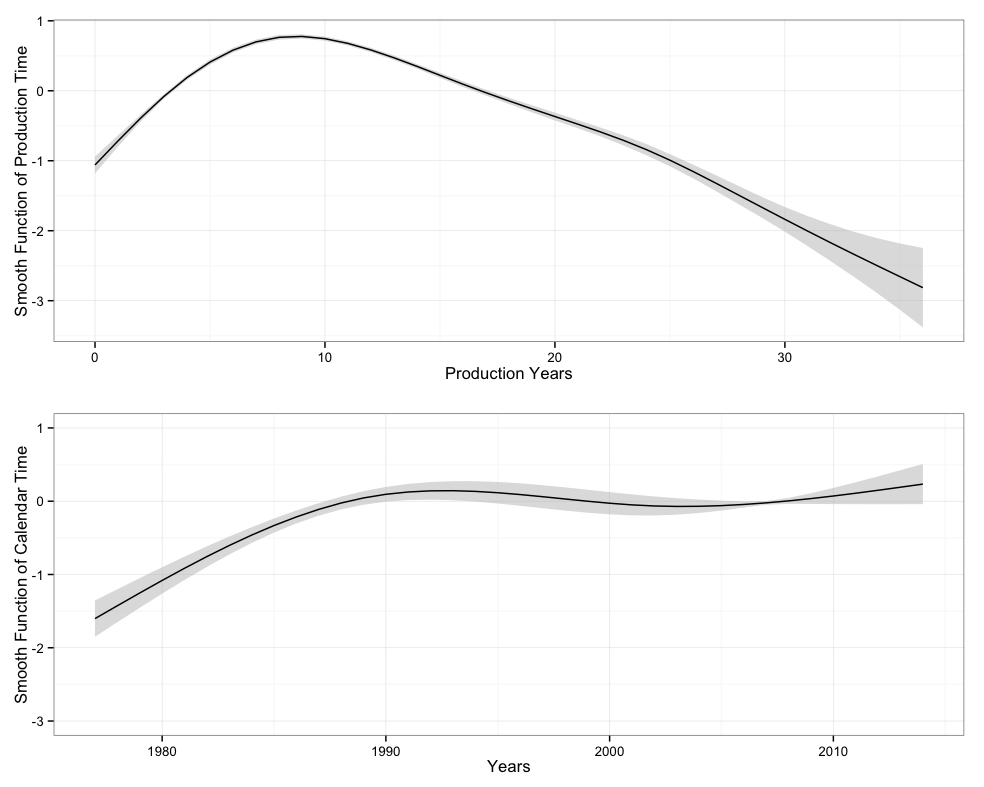
\includegraphics[width=1\textwidth]{figures/smooths.png}
	\caption{The estimated smoothed functions over production time and calendar time.}
	\label{smooths}
\end{figure}

One objection to the simple model is that a fixed effect controlling for the general production profile of oil fields does not sufficiently take into account the idiosyncratic variance between the fields. To address this I can add field random effects that take into account uncertainty based on random variation between the fields in the estimation. The smoothed function can then be written as $f(production\_time_{i,t}*Z)$.  Where $Z \sim N(0, \sigma)$ and $\sigma$ is the variance term to be estimated.  

Another potential issue may be that the smoothed function of production time may not be sufficient in controlling for the variation in production profiles shapes across fields.  In particular, production profiles differ substantially by the size of the field. A solution is to allow the shape to vary by the size of the field - here I use an estimate of in-place oil in the field rather than recoverable reserves, as recoverable reserves may be correlated with oil prices.  Thus the smoothed term can be written as a function of both production time and in place oil: $f(production\_time_{i,t}, in\_place\_oil_{i})$.

Estimating a smoothed function of two variables requires a somewhat more involved method.  In particular, a thin-plate regression spline \citep{wood_thin_2003} is used. Consider equation \ref{thin_plate_1}. 

	\begin{equation}
	y_i = g(x_1, x_2)
	\label{thin_plate_1}
	\end{equation}

Following the notation of \citet{wood_generalized_2006}, $g$ is the function of $x_1$ and $x_2$ that is to be estimated by $f$, which in turn is estimated by minimizing equation \ref{thin_plate_2}.  Here $\boldsymbol{y}$ represents a vector of $y_i$'s and $\boldsymbol{f} = (f(\boldsymbol{x_1}),f(\boldsymbol{x_2}))^t$.   

	\begin{equation}
\min \|\boldsymbol{y-f}\|^2 + \lambda J_{22}(f)
\label{thin_plate_2}
	\end{equation}

$J_{22}$ represents the penalty term for the smoothness of the function, which can be written as in \ref{thin_plate_3}.  The $22$ represents the fact that it is a penalty function of two variables with smoothness measured by the second derivative.

	\begin{equation}
	J_{22}(f)= \Big(  \diffp[2]{f}{x_1} \Big)^2 +
	 \Big(\frac{\partial^2 f}{\partial x_1 \partial x_2}\Big)^2 + 
	\Big(\diffp[2]{f}{x_2} \Big)^2dx_1 dx_2
\label{thin_plate_3}
	\end{equation}

In short, a function of $x_1$ and $x_2$ is found that is minimizing errors in the sense of minimizing Euclidean distance subject to a penalty function of “wiggiliness”.  The actual implementation is somewhat more involved in order to increase the computational efficiency of the estimation.  For further technical details I refer to \citet{wood_thin_2003}. 

Unfortunately, estimating a random effects component is not possible with a two-dimensional smoothed function for computational reasons.  In the presentation of results, I therefore present models side-by-side that use both one-dimensional smooth functions with random effects of the field production profile and two-dimensional smooth functions.

In general I assume that oil prices are exogenous in this model. On the supply side, oil is a globally traded commodity.  Since I am measuring changes in production at the field level, these are highly unlikely to have any effect on global oil prices.

A more subtle possibility for endogeneity exists on the demand side. A bias could result if demand also was correlated with changes in field production other than through the direct price-mechanism. For example, higher GDP could mean easier lending to petroleum companies, who then might invest and increase petroleum production independent of higher oil prices. I investigated this by including a measure of world GDP growth obtained from the World Bank in the regression. Using an F-test, adding this variable could not be shown to significantly increase the fit of the model, suggesting that demand-side effects are unlikely to be causing a bias. I therefore exclude this variable from the results presented below.

\section{The Effect of Oil Price on Field Production}

Table \ref{GAM_model_table} shows the estimated parametric coefficient terms and other summary statistics of the regression results.  The first column shows results for the simple model with a single-dimensional smoothed function of the production profile.  The second column shows results with field-level random effects, while the third columns shows results when a two-dimensional smoothed function is used to control for production profiles across field sizes. The latter two models are my preferred models, providing a substantially better fit, as measured by both deviance explained and $R^2$. Monte Carlo experiments, which I describe further below, also indicate that the latter two models provide consistently less-biased parametric estimates of the price terms. This is especially the case for the model with a 2-dimensional smoothed term.

The variables of interest in this article is the oil price and its lags, which I include as eight linear parametric terms in the model.  The reason for including both a concurrent oil price term as well as eight lags is that a change in price could conceivably have two effects on oil production in a field.  First, the field operator could be operating on the basis of some short-term extraction rule - choosing to pump out less at times of lower prices in order to pump out more at periods of high prices.  

Alternatively, a change in the price of oil can be seen as a lifting of a production constraint.  A higher oil price means that added investments in production becomes attractive in order to either increase the total amount extracted from a field or to shift production forward.  However investments in the offshore sector can be complex and lengthy, and any production lift would be expected to happen with a lag.  As mentioned earlier, including several lags also allows for the possibility of adaptive expectations of future oil prices.  

\begin{table}
\scriptsize
\begin{center}
\begin{tabular}{l c c c c }
\hline
 & w/out Rand. Effects & w Rand. Effects & 2-d Smooth & w Build-out \\
\hline
Intercept                                  & $0.335$        & $-4.016^{***}$ & $-574.287^{***}$ & $-3.858^{***}$ \\
                                             & $(0.265)$      & $(0.297)$      & $(89.476)$       & $(0.239)$      \\
in\_place\_oil             & $0.337^{***}$  & $-0.014$       &                  & $-0.015$       \\
                                             & $(0.009)$      & $(0.022)$      &                  & $(0.024)$      \\
cost\_index                            & $-0.018^{**}$  & $-0.030^{***}$ & $-0.014^{***}$   & $-0.034^{***}$ \\
                                             & $(0.006)$      & $(0.006)$      & $(0.004)$        & $(0.006)$      \\
price                                  & $-0.006$       & $0.014$        & $0.007$          & $0.005$        \\
                                             & $(0.017)$      & $(0.016)$      & $(0.011)$        & $(0.015)$      \\
price\_l1                              & $0.004$        & $0.021$        & $0.015$          & $-0.003$       \\
                                             & $(0.017)$      & $(0.017)$      & $(0.011)$        & $(0.020)$      \\
price\_l2                              & $0.037^{*}$    & $0.047^{**}$   & $0.048^{***}$    & $0.053^{*}$    \\
                                             & $(0.017)$      & $(0.016)$      & $(0.011)$        & $(0.023)$      \\
price\_l3                              & $0.030$        & $0.025$        & $0.033^{***}$    & $0.017$        \\
                                             & $(0.016)$      & $(0.014)$      & $(0.010)$        & $(0.024)$      \\
price\_l4                              & $0.003$        & $0.043^{**}$   & $0.028^{**}$     & $0.076^{***}$  \\
                                             & $(0.015)$      & $(0.014)$      & $(0.009)$        & $(0.020)$      \\
price\_l5                              & $-0.020$       & $0.012$        & $-0.001$         &                \\
                                             & $(0.013)$      & $(0.012)$      & $(0.008)$        &                \\
price\_l6                              & $-0.010$       & $0.008$        & $-0.001$         &                \\
                                             & $(0.012)$      & $(0.011)$      & $(0.008)$        &                \\
price\_l7                              & $-0.008$       & $0.007$        & $0.004$          &                \\
                                             & $(0.012)$      & $(0.012)$      & $(0.008)$        &                \\
price\_l8                              & $-0.044^{***}$ & $-0.011$       & $-0.027^{***}$   &                \\
                                             & $(0.011)$      & $(0.011)$      & $(0.007)$        &                \\
EDF: s(prod\_year)                           & $6.381^{***}$  &                &                  &                \\
                                             & $(7.249)$      &                &                  &                \\
EDF: s(year)                                 & $2.768^{***}$  & $3.000^{***}$  & $3.000^{***}$    & $3.000^{***}$  \\
                                             & $(2.956)$      & $(3.000)$      & $(3.000)$        & $(3.000)$      \\
EDF: s(prod\_year,name)                      &                & $33.002^{***}$ &                  & $32.962^{***}$ \\
                                             &                & $(72.000)$     &                  & $(72.000)$     \\
EDF: s(prod\_year,in\_place\_oil) &                &                & $27.445^{***}$   &                \\
                                             &                &                & $(27.895)$       &                \\
price\_l1:build\_out                   &                &                &                  & $0.038$        \\
                                             &                &                &                  & $(0.024)$      \\
price\_l2:build\_out                   &                &                &                  & $-0.002$       \\
                                             &                &                &                  & $(0.029)$      \\
price\_l3:build\_out                   &                &                &                  & $0.003$        \\
                                             &                &                &                  & $(0.029)$      \\
price\_l4:build\_out                   &                &                &                  & $-0.027$       \\
                                             &                &                &                  & $(0.024)$      \\
\hline
Deviance                                     & 23062.678      & 19765.852      & 9057.204         & 19786.567      \\
Deviance explained                           & 0.848          & 0.870          & 0.940            & 0.870          \\
Dispersion                                   & 17.852         & 15.625         & 7.123            & 15.641         \\
R$^2$                                        & 0.841          & 0.865          & 0.938            & 0.865          \\
GCV score                                    & 18.145         & 16.218         & 7.355            & 16.234         \\
Num. obs.                                    & 1088           & 1088           & 1088             & 1088           \\
Num. smooth terms                            & 2              & 2              & 2                & 2              \\
\hline
\multicolumn{5}{l}{\scriptsize{$^{***}p<0.001$, $^{**}p<0.01$, $^*p<0.05$}}
\end{tabular}
\caption{Model results. Estimated coefficients are shown for the linear terms. Standard errors are in parenthesis. For the smoothed terms, estimated degrees of freedom are displayed, where the p-values are from F-tests of whether the smooth terms significantly improve the fit of the model.}
\label{GAM_model_table}
\end{center}
\end{table}

 
For convenience the estimated coefficients on the price terms from the two preferred models are shown in figure \ref{price_coefficients}. In general the results from the two models agree with each other, indicating little to no effect on the concurrent price term, but with positive coefficients estimated on the 2st to 4th lags, with a peak at the 2nd lag. A negative coefficient for the eighth lag is estimated in the 2-d model, however this is not significant in the model with random effects. Furthermore, F-tests with comparisons to restricted models without the concurrent and 5-8th lags indicate that these terms do not as a group significantly improve the fit of the model. On the other hand, the block of terms for the 1st through 4th lags do significantly add to the fit of the model.

\begin{figure}
	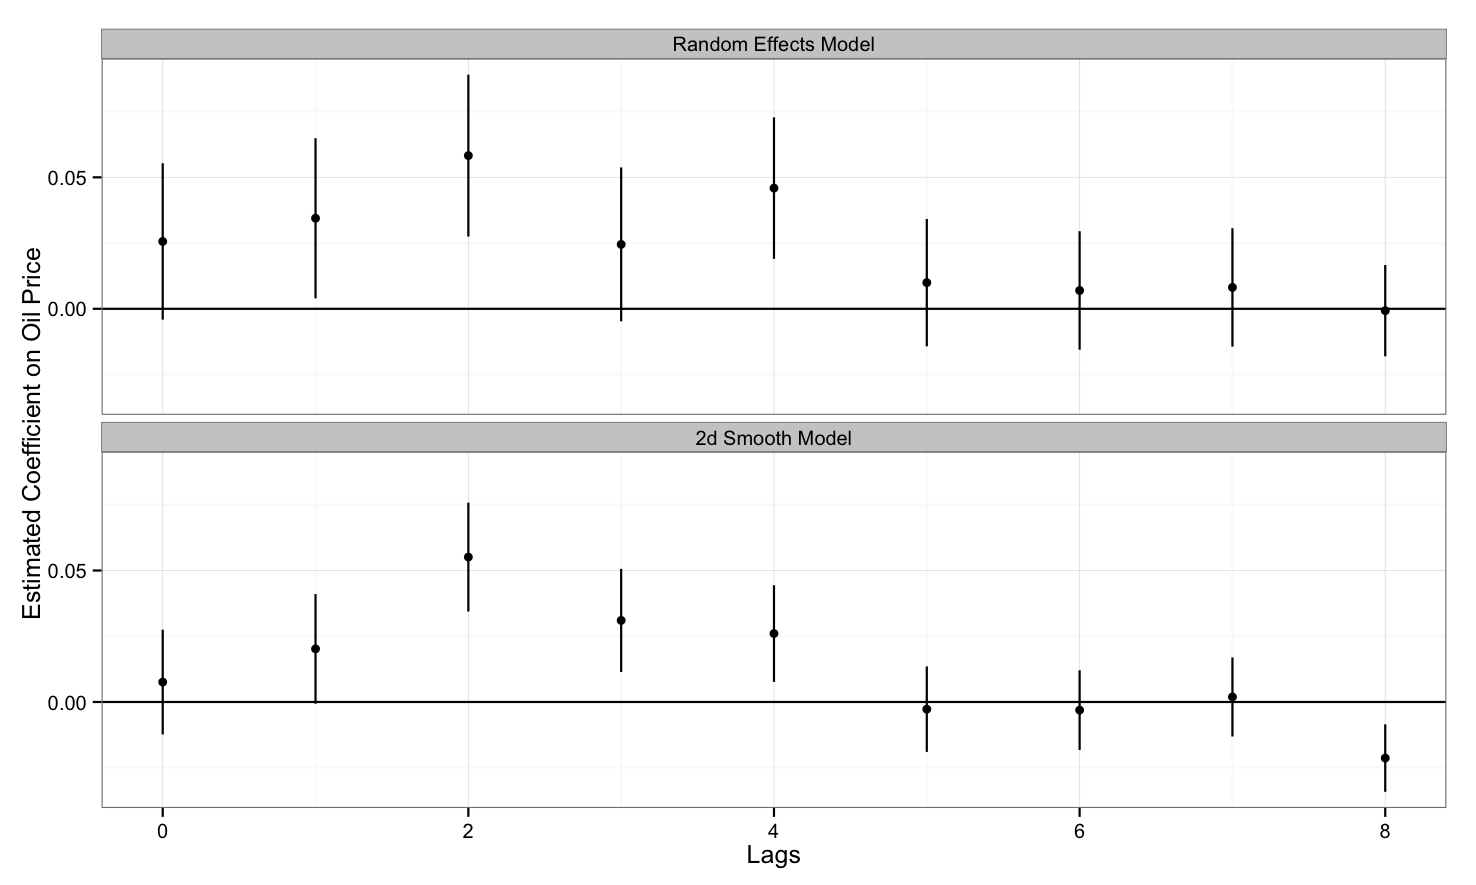
\includegraphics[width=1\textwidth]{figures/price_coefficents.png}
	\caption{Estimated coefficients from two GAM models: a model with random field effects and single smoothed function of production time, and another with a two dimensional smoothed function of production time and field size.  The points represent the point estimates, while the lines represent approximate 95\% confidence intervals. Significant positive coefficients are estimated on lags of between 2-4 years.  However, little to no effect is measured on the concurrent price term.}
	\label{price_coefficients}
\end{figure}

One potential weakness of the estimation so far is that I do not take into account the different stages of field production, where the effect of price could be expected to differ. 
In particular, in the build-out phase of a field, where production is started and then ramped up to full capacity, the field operator has an incentive to build out the field as quickly as possible as large amounts of capital have at that point been allocated and it is important to get oil production and in turn income flowing. At this stage, it is ex-ante questionable that prices would have an effect on production, as a decision to increase capacity would require a new submission to the regulators and a potentially lengthy and expensive delay. On the other hand, the draw down phase is characterized by overcapacity and in turn greater flexibility in increasing production by way of, for example, infill drilling that can both accelerate recovery and increase total recovery in a field. \footnote{I thank an anonymous referee for making this point.}

To attempt to capture this heterogeneity, I introduce an indicator variable that represents the build-out phase defined as the period between the start of production up to peak production. I add interaction effects between this indicator variable and the block of significant lagged price effects $price\_l1$ through $price\_l4$.

The main problem with introducing this heterogeneity in the model is that most field build-outs happen quickly, usually within one or two years in most small to medium sized fields. The sample to estimate the build out price terms is then relatively small - less than one third of the total observations. The small sub-sample leads to estimation problems when using the model with a 2-dimensional smooth term, so I instead extend the random effects model. I also remove the block of 5th through 8th year lagged price terms that could not be shown to increase the fit of the model.

The estimation results for this model are shown in the fourth column of table \ref{GAM_model_table}. The interaction effects, labeled $price\_lt:build$, are not estimated to be significantly different from zero. Given the small sample used to estimate these terms, this is not surprising. On the other hand, if we compare the main effects of the lagged price terms to the standard random effects model, we notice that the point estimates on the 2nd, 3rd and 4th lags are now subsantially larger in magnitude. In this model, these main effect terms can be interpreted as the effect of price on production in the draw-down phase. This provides some evidence that the effect of price on production is indeed strongest in this latter stage of field development.

For computationally intensive Generalized Additive Models, few if any analytic results are available to confirm that the estimates are unbiased.  Instead, I rely on Monte Carlo experiments to test for bias.  Here, I create artificial field data using a cumulative logistic function with a linear price term and random variation. I then estimate the effect of price repeatedly, generating the random component before each new estimation. Details of the Monte Carlo experiment can be found in the on-line appendix \url{https://github.com/jmaurit/oil_prices/blob/master/mc_sim.pdf}.  

The main results are shown in figure \ref{mc_results}.  The top panel shows one run of the artificially generated data. I compare estimations of a concurrent price term, $beta\_hat$ made with a Generalized Linear Model and Generalized Additive Model with a 2-dimensional smooth function.  I set the true parameter $beta$ to both $0$ and $0.05$, which are shown as vertical lines in the figures.  The figure shows that while a bias exists in the estimation of the GLM model, especially for when the true value is $0.05$, the Generalized Additive Model generally provides unbiased results. 

\begin{figure}
	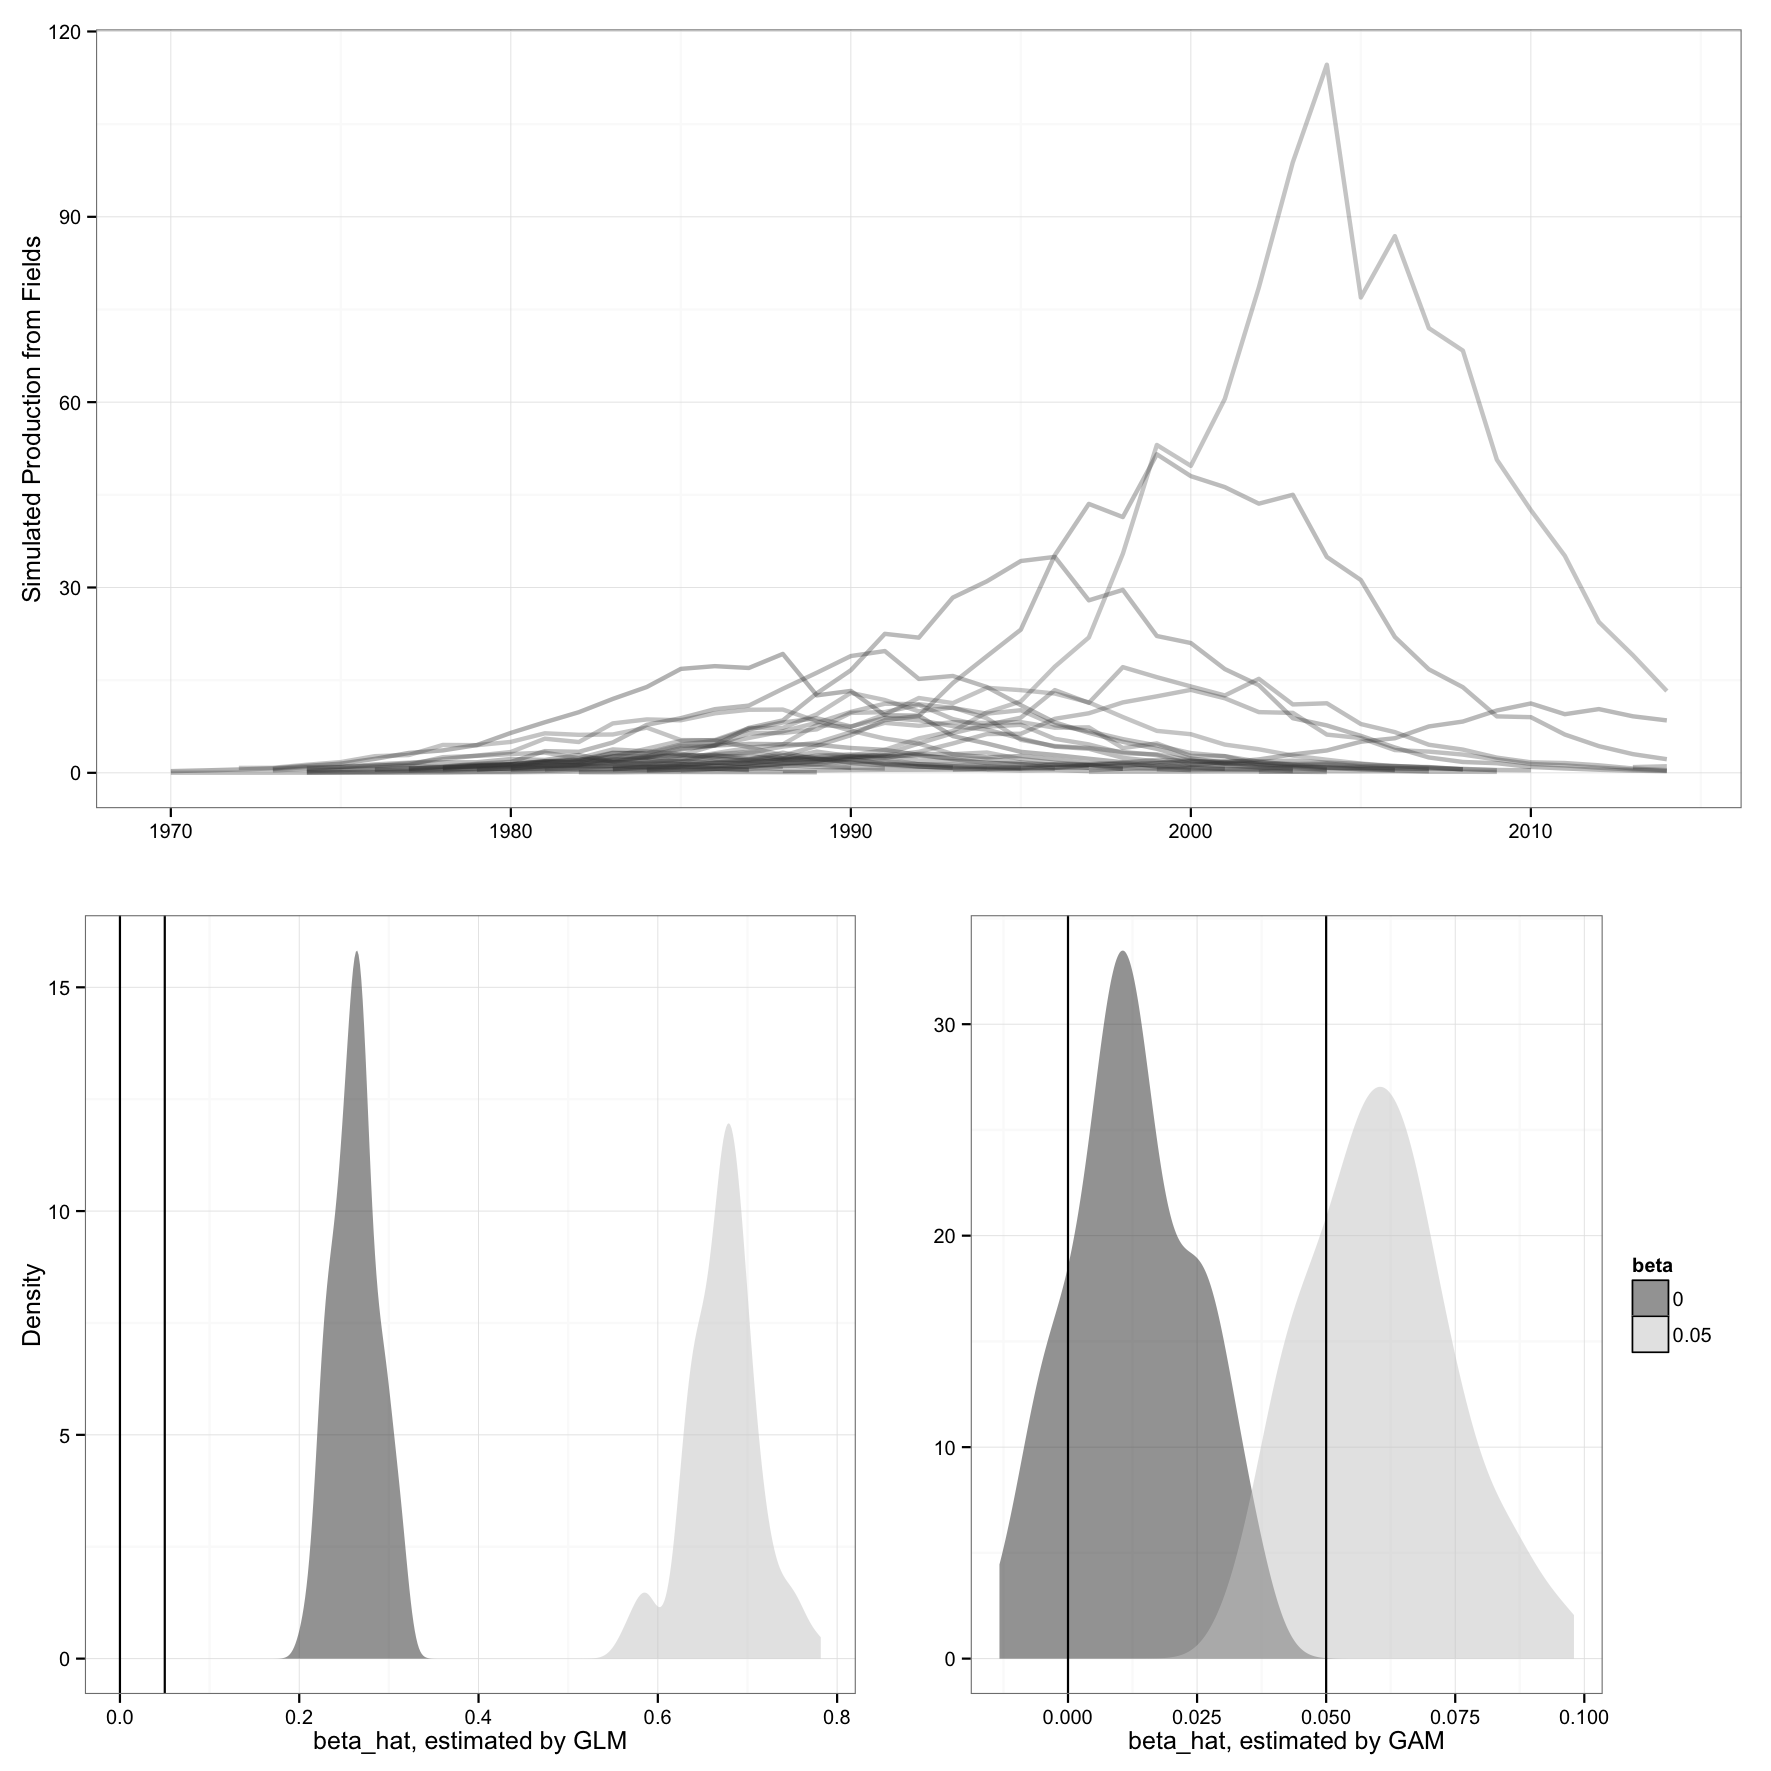
\includegraphics[width=1\textwidth]{figures/mc_plot.png}
	\caption{Results from a Monte-Carlo experiment. I generate data mimicking oil price production from a set of fields, as displayed in the top frame. Using GLM and GAM models, and regenerating the error component in the data, I replicate estimates of the effect of price on production, which is set at $\beta = 0$ and $\beta=0.05$. The density of the results for the GLM model are shown in the lower left panel, where a clear and large bias is shown relative to the true $\beta$ which are represented by the vertical lines.  A GAM model however provides estimates close to the true $\beta$}
	\label{mc_results}
\end{figure}

\section{Conclusion and Discussion}

The main result of this research is to show that production in existing Norwegian offshore fields has no significant concurrent reaction to higher oil prices while a modest effect is estimated  with a lag of between 2 and 4 years.  Oil producers do not appear to be behaving strategically in relation to short-term production - increasing or reducing production in response to changes in oil price.  Instead they are likely using storage or financial instruments to hedge short-term price movements. Changes in oil prices can rather be seen as a relaxing of a production constraint, justifying increased investment that leads to either a higher total extraction rate or an inter-temporal shifting of production.

One important caveat is that I do not claim to capture all possible mechanisms for price to influence production.  Mechanisms that are likely gradual and smooth in nature will be absorbed by the smooth functions in the regression. In particular, price-induced technological change will likely be a smooth process with significant lag times. Referring back to figure \ref{smooths}, some evidence of this can perhaps be seen in the estimated smooth function of the calendar year variable, which shows a slight (and statistically insignificant) upwards slope after approximately 2005, corresponding to a preceding period of rising oil prices.   

Another important caveat is that the changes in production could potentially either be a permanent increase in production, or a shift forward of production that may otherwise have happened later. Unfortunately, with the existing data and methods, I do not see a good way of distinguishing between these alternatives. First, there is the problem of censored data, as most of the fields in the data set are still producing, thus the information on how long the fields eventually produce are not available.  More so, the estimates of both recoverable reserves and in-place oil are too uncertain in order to to make calculations of whether a change in production in one period led to a reduction in another - especially when the changes in production are relatively modest.

Interpreting the lagged effects also involves some subtlety. As noted, evidence has been found for adaptive expectations of future oil prices.  Thus, the lagged effects could be interpreted as both the result of investment lags as well as lags involved in updating of expectations. Completely disentangling these effects would probably at a minimum require a structural model with some specific assumptions about the formation of expectations, which is beyond the scope of this article. 

However, the magnitude and the ordering of the estimated price effects indicates that investment lags are likely dominant. Since the current price always contains the most up-to-date information, then a model of adaptive expectations would show the largest effect at the concurrent term, thereafter receding. The estimations in this article however can show no significant concurrent effect, with the largest magnitude effect consistently being estimated at a 2-year lag.

The findings in this article can provide some guidance on predicting the effects of the recent steep fall in the oil price on Norwegian production, as well as production from other offshore production areas. The results suggest that lower oil prices are likely to have only modest ramifications for production in existing fields.  Anecdotal evidence however suggests that searching and exploration are being substantially curtailed. Future oil production could then be significantly affected by way of fewer new field developments.

Policy implications arise for both energy industry regulators and financial policy makers. Since the evidence points to a stronger lagged effect of price on production in declining fields, this would also imply that policy measures meant to stimulate increased production would likely also be more effective in mature oil producing areas compared to newer areas. This is particularily important on the Norwegian Continental Shelf, as several new fields have recently come online following a period of high oil prices. \footnote{I thank an anonymous reviewer for pointing out this implication.}

Finally, relating back to the literature on total oil supply, the modest estimated effect of prices on production adds weight to the argument of \citet{hamilton_oil_2012} that most of the increased supply of oil that comes from higher prices is from expanding the geographic and technological boundaries of oil production.  For example exploration of deep-water oil deposits off the coast of Brazil and extraction of oil sands in western Canada.

\FloatBarrier
\section{Software}
I use the R statistical programming package for all the analysis in this article \citep{r_core_team_r:_2013}.  I use the R package ggplot2 for plotting \citep{wickham_ggplot2:_2009}, plyr for data manipulation and cleaning \citep{wickham_split-apply-combine_2011}, texreg for table formatting \citep{leifeld_texreg:_2013} and mgcv for implementation of the Generalized Additive Models \citep{wood_fast_2011}.

\section{Acknowledgments}
I thank Klaus Mohn, Jonas Andersson, Sturla Kvamsdal, Harrison Fell, R\"ognvaldur Hannesson and Henrik Horn for valuable discussion. I have received financial support from the Norwegian Center for Sustainable Energy Studies (CenSES), Norwegian Research Council grant number 209697 

\begin{spacing}{1}
\bibliographystyle{plainnat}
\bibliography{oil_prices}
\end{spacing}

\end{document}